\begin{CJK}{Bg5}{bsmi}

%---------------------------------------------
%	Chapter Discussion
%---------------------------------------------

\chapter{Discussion}

\section{Security Analysis}

\begin{comment}
This is the most important part of an authentication system.
We have to define our threat model before we start to analyze.
There are 4 components in the scheme I proposed.
\end{comment}

\subsection{Threat Model}

There are 5 components in the scheme I proposed, as the fig~\ref{fig:compose-element} shows.

\begin{figure}
\centering
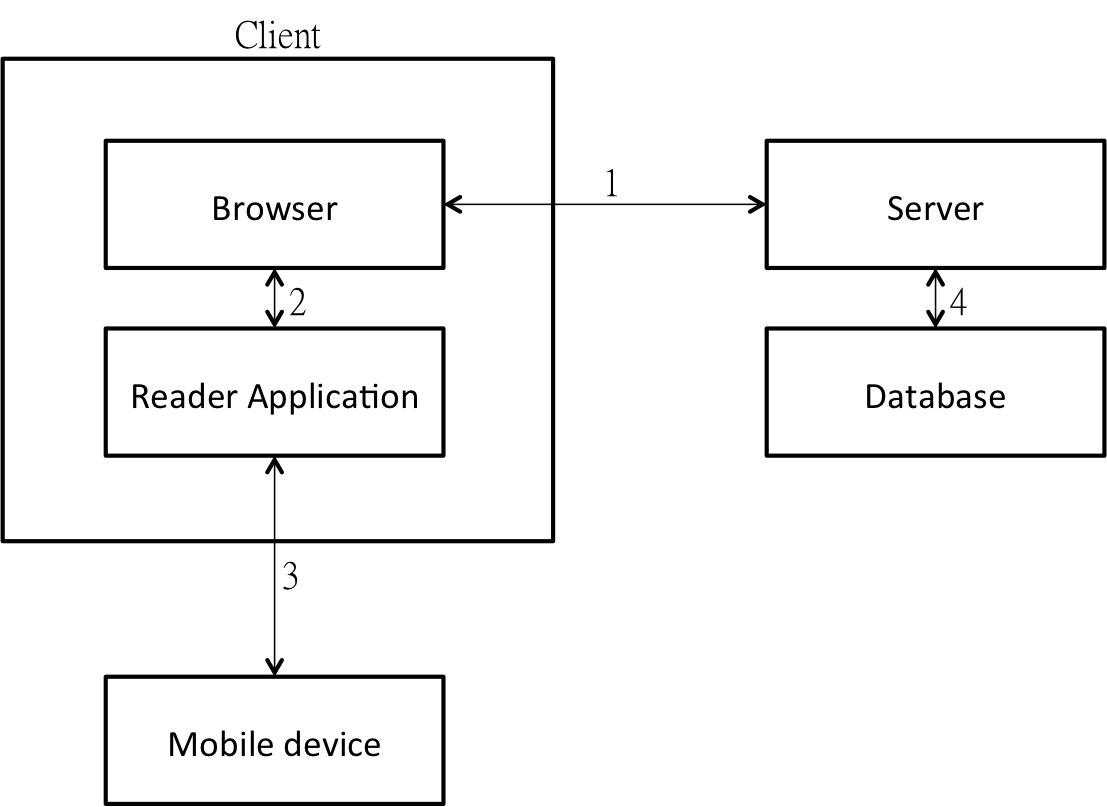
\includegraphics[scale=0.6]{picture/compose-element.png}
\caption{Components}
\label{fig:compose-element}
\end{figure}

\subsection{Analysis}

\section{Usability Analysis}

\subsection{Criterias}

\subsubsection{Memorywise-effort}

This criteria means that how many things a user has to remember when he adopt this scheme. Take password-based scheme as an example, the memorywise-effort is username and password. A scheme with less memorywise effort can get higher score in this criteria.

\subsubsection{Scalable-for-user}

Will this scheme create burden for users? The \emph{scalable} is from the viewpoint of users.

\subsubsection{Nothing-to-carry}

Users do not need to bring anything if they adopt this scheme.

\subsubsection{Physical-effortless}

This criteria means that how many effort should a user do in an authentication process.

\subsubsection{Efficiency}

Efficiency means the during time of an authenticaiton process. Not only the calculating time, it should also include the operating time. For example, if a user need to enter an OTP himself, then this scheme is not efficiency.

\subsubsection{Infrequent-error}

Infrequent-error means this scheme or system must be reliable. It cannot reject an authentication request to a honest user.

\subsubsection{Easy-recovery-from-loss}

Users can regain the authentication ability if they lost their devices or if they forgot the needed credentials.

\subsection{Analysis}

\begin{comment}
The usability can not be neglected when researchers trying to design a system.
Usability is a subjective perception, it may be different from person to person.
The following paragragh states the criterias I used to estimate the usability of a system.
\end{comment}

\section{Deployment Ability Analysis}

\subsection{Criterias}

\subsubsection{Accessible}

User who adopt this scheme will not be constrained by disabilities or any other physical conditions.

\subsubsection{User-cost}

The total cost per user of the scheme. It should including both required devices of client-side and required equipment of the verification server.

\subsubsection{Server-compatable}

From the viewpoint of verification server, the scheme is compatable with the text-based passwords. The server will not need change their setup to support this scheme. 

\subsubsection{Browser-compatable}

Users don't have to change anything to support this scheme. 

\subsection{Analysis}

\begin{comment}
The deployment ability is also an important thing which is need to be considered, especially in designing an authentication system.
A system with high usability means it is friendly to users; a system with high deployment ability means it is friendly to the system provider or, more precise, the developers.
The following paragraph states the criterias I used to estimate a system's deployment ability. 
\end{comment}


\end{CJK}